\documentclass[tikz,border=5pt]{standalone}
\usepackage{pgfplots}
\pgfplotsset{compat=1.18}
\usepackage{fontspec}
\setsansfont{SourceSansPro}[
  Path = /usr/local/texlive/2024/texmf-dist/fonts/opentype/adobe/sourcesanspro/,
  UprightFont = SourceSansPro-Regular.otf,
  BoldFont = SourceSansPro-Bold.otf,
  ItalicFont = SourceSansPro-RegularIt.otf,
  BoldItalicFont = SourceSansPro-BoldIt.otf,
  Scale = 1.0
]
\usetikzlibrary{positioning}
\usepackage{xcolor}
\definecolor{primaryblue}{HTML}{012169}
\definecolor{primarygold}{HTML}{B9975B}
\definecolor{highlightyellow}{HTML}{F2A900}
\definecolor{lightbg}{HTML}{E8EDF5}
\definecolor{jet}{HTML}{1A1A1A}
\definecolor{positivegreen}{HTML}{15803D}
\definecolor{negativered}{HTML}{B91C1C}
\begin{document}
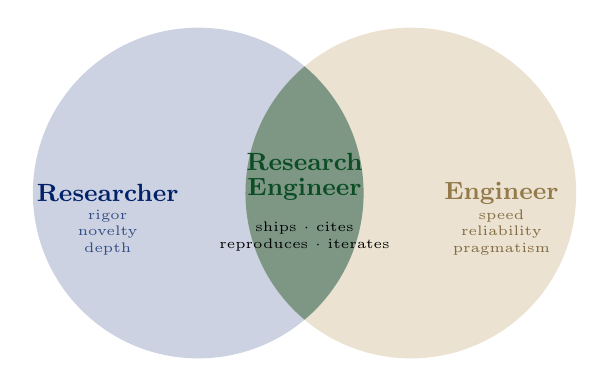
\begin{tikzpicture}
  \begin{scope}[blend mode=multiply]
    % Left circle: Researcher
    \fill[primaryblue!25, opacity=0.8] (-1.35,0) circle (2.1cm);
    % Right circle: Engineer
    \fill[primarygold!35, opacity=0.8] (1.35,0) circle (2.1cm);
    % Overlap: Research Engineer (highlighted)
    \begin{scope}
      \clip (-1.35,0) circle (2.1cm);
      \fill[positivegreen!40, opacity=0.9] (1.35,0) circle (2.1cm);
    \end{scope}
  \end{scope}
  % Labels
  \node[font=\small\bfseries, text=primaryblue] at (-2.5,0) {Researcher};
  \node[font=\tiny, text=primaryblue!80, align=center] at (-2.5,-0.5)
    {rigor\\novelty\\depth};
  \node[font=\small\bfseries, text=primarygold!80!black] at (2.5,0) {Engineer};
  \node[font=\tiny, text=primarygold!70!black, align=center] at (2.5,-0.5)
    {speed\\reliability\\pragmatism};
  \node[font=\small\bfseries, text=positivegreen!60!black] at (0,0.4)
    {Research};
  \node[font=\small\bfseries, text=positivegreen!60!black] at (0,0.05)
    {Engineer};
  \node[font=\tiny, text=black, align=center] at (0,-0.55)
    {ships $\cdot$ cites\\reproduces $\cdot$ iterates};
\end{tikzpicture}
\end{document}
